%%%%%%%%%%%%%%%%%%%%%%%%%%%
%%%%%%INTRODUCTION%%%%%%%%
%%%%%%%%%%%%%%%%%%%%%%%%%%%
	\section{Motivation}
	
	To these days, and since long time ago financists, economists, statisticians tried to figure out an exact method 
	to predict the fluctuations of the price based mostly on its history. This methods are quite accurate in ideal
	conditions. If we recall the financial crisis that happen in the 2008 (\cite{P2009}, \cite{R2010}); of course, this is not a normal situation of any 
	market. The forecasts said something while the actual numbers where not reflecting what was predicted. 
	
	The aim of this thesis is not to develop a new method in order to predict the price of a stock, or to tell an investor to buy
	or not to buy. But to realise how qualitative aspects (what is written on the news) could somehow affect the changes in the price of a stock.
	
	Initially we will assume the most natural position: That the positive news are positively correlated with the 
	positive increments of the stock and vice-versa: the negative news are positively correlated with the drops
	in the stock prices.
	
	\clearpage
	\section{Main Goals}
	
	As previously mentioned in the Motivation, we will focus on the qualitative part of the companies, therefore the main goal of the thesis is to define and realise a tool for collecting, analysing and summarising qualitative information about companies left in news articles. 
	We must clarify that with the term \emph{"Analysis"}, we mean a \emph{Polarity or Sentiment Analisys}.
	
	We will create a \emph{crawler}, which initially will get a "link seed" and then it will go through specific links. After this, the crawler will extract and save the content of the page.
	
	Once we have downloaded and extracted the article with the \emph{crawler}, we will proceed to analyse its polarity; then we will assign a score to the document, and according to this score we will define if it has positive or negative polarity.


	\section{Problem statement}
	
	The main sight of this thesis is to  provide a \emph{Framework} to retrieve, analyse and summarise data from news articles in order to provide qualitative information about some particular company.

	\clearpage
	\section{State of the Art}
	
	The main goal of our project is to consider not only quantitative (stock price of a company, ratios, etc.) factors about the stock market, but to consider the qualitative part (News articles mostly) in order to analyse what are the trends of the qualitative aspects.

	To perform this analysis we will use several techniques and algorithms (Web crawlers and Sentiment Analysis), we will be mentioning the highest level of development of this techniques until today. We will help ourselves with some part of a thesis written by Avni Gural \cite{V2013}, in order to describe the state of the art of our techniques and algorithms.
	
	\subsection{Web Crawlers}
	
	According to Gural \cite{V2013} a web crawler, also known as harvester, spider, or robot, is an application that browses the World Wide Web and automatically downloads web pages and also can be used for gathering specific information, like in our case; news articles. The main part of such a basic crawler is the download queue(or sometimes referred as frontier). A specialised version of crawling, called focused web crawling, is proposed aiming to collect on-topic data which actually reduces the search space.
			
	Web crawling has many challenges. As stated by Najork \cite{N2009}, a web-scale web crawler imposes major engineering challenges, all of which are ultimately related to scale. A typical crawler has to fetch thousands of pages in a second in order to maintain a fresh corpus of search engine with a couple of billion pages. We can observe in the figure \ref{fig:Crawler_001} the basic architecture of a web crawler.
	
	\begin{figure}\centering
		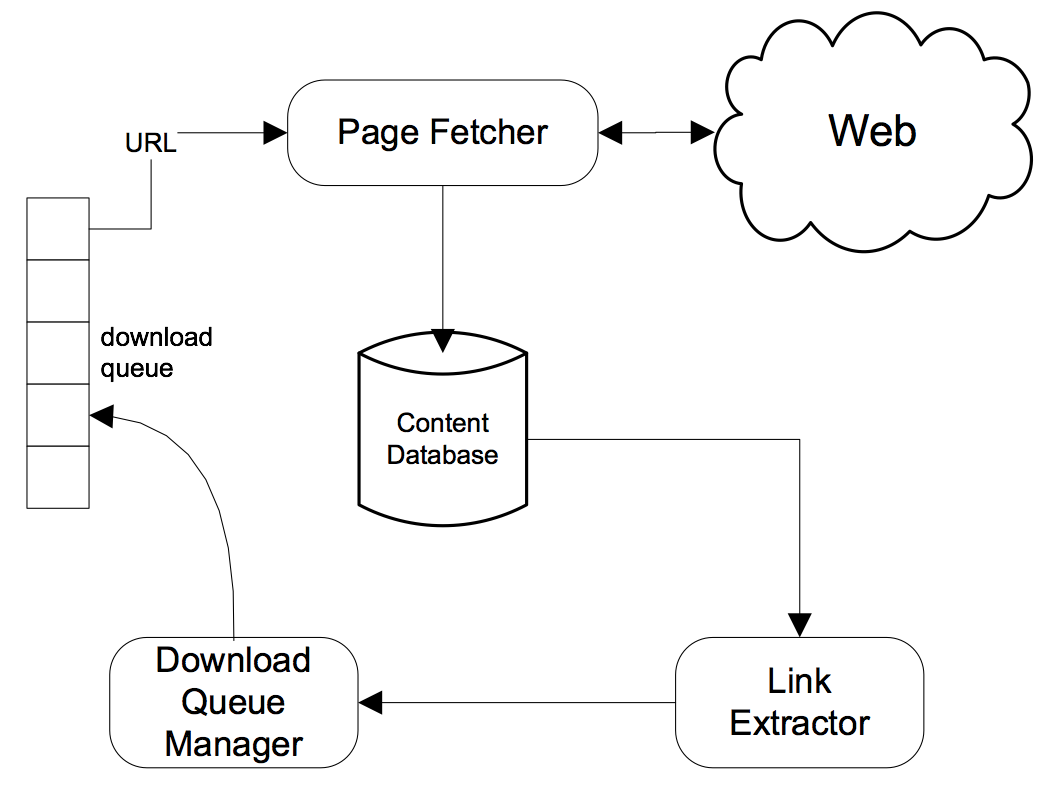
\includegraphics[scale=0.3]{Crawler_001}
		\caption{Basic web crawler algorithm.}\label{fig:Crawler_001}
	\end{figure}
		
	\begin{itemize}
		\item Content Selection: Crawlers should bypass irrelevant, low-quality, malicious content.
		\item Scale: Web hosts an enormous amount of data but the crawlers seek broad coverage and freshness.
		\item Speed: The basic and fast way of keeping track of visited URLs is storing in the memory. However, it is not possible to store hundreds of millions of URLs in the memory. That is why such lists are kept on disk, but accessing and re-ordering the list becomes slower and degrade the crawling performance.
		\item Infrastructure Cost: According to a blog post on the Official Google Blog \cite{A2013}, the Google index now contains about 1 trillion unique URL's. This graph of one trillion URLs is similar to a map made up of one trillion intersections, which is continuously reprocessed several times per day. Storing, indexing and fresh-keeping such a huge data requires massive investments on hardware infrastructure.
		\item Ethics / Politeness: Crawlers should prevent server overload and comply with Robot Exclusion Protocol according to Koster in his article \cite{K2013}: \emph{"A standard for robot exclusion."}(which is a de facto standard for definition of access rights on a website for crawling).
	\end{itemize}
	
	\subsubsection{Focused Web Crawling}\label{focusedWebCrawling}

	One of the most important properties of a crawler is the speed; this becomes even more important when we think about the web hosting an enormous amount of data in various forms, structures, formats, etc. Is estimated to have more than 10 billion pages and continues to grow rapidly according to the work of Kunder \cite{WWW2013}. 
	
	
	Crawlers should discover and use not only the new pages but also the recent versions of the pages. A general purpose crawler is said to be neither necessary nor sufficient to crawl and index such a giant amount of web pages. Therefore, a specialised version of crawling, called focused web crawling, is proposed aiming to collect on-topic data which actually reduces the search space.
	
	The first related work on focused crawling was done by De Bra in his article \emph{"Information retrieval in distributed hypertexts"} \cite%[p. 481-493]
	{B1994}, called fish search. In this research, for a client-based search engine, a simulated group of fish crawls on the web and assigns page relevance metric to pages using a binary classification with an input of simple keyword or regular expression. The lifespan of a fish depends on visited page relevance, where the fish dies when a specified amount of irrelevant pages are traversed. In addition, a fish produces offspring when a new page is traversed. Fish search works as depth-first search, since new URLs are added to the beginning of the download queue.
	
	Later, an extended version of fish search was developed, so called shark search, it was proposed by Hersovici in his article: \emph{"The shark-search algorithm"} \cite%[p. 317-326]
	{H1998}. In contrast to fish search, shark search estimates page relevance with a continuous function resulting a real number between 0 and 1 for the a similarity between document and query. Then, in the download queue, URLs are ordered by linear combination of source page relevance, anchor text and neighbourhood of the link on the source page.

	\subsection{Sentiment Analysis}
	
	Opinions as the key influencers of our behaviour are important. As Liu \cite%[p. 459-460]
	{L2011} stated, our beliefs and perceptions of the reality, and the choices we make, are susceptible on how others see and evaluate the world. This is the reason why people seek out opinions of others when making a decision. Sentiment analysis (a.k.a. opinion mining) is an area of study and analysing people's opinions, appraisals, attitudes, feelings, and emotions toward entities, individuals, issues, events, topics and their attributes. Sentiment analysis has been an active research area for quite some time. Feldman \cite%[p. 82-89]
	{F2013} states that there are over 7,000 articles on the topic of sentiment analysis, and apart from the techniques applied, all sentiment analysis systems implement a generic pipeline, which is illustrated in Figure \ref{fig:Sentiment_001}.
	
	\begin{figure}\centering
		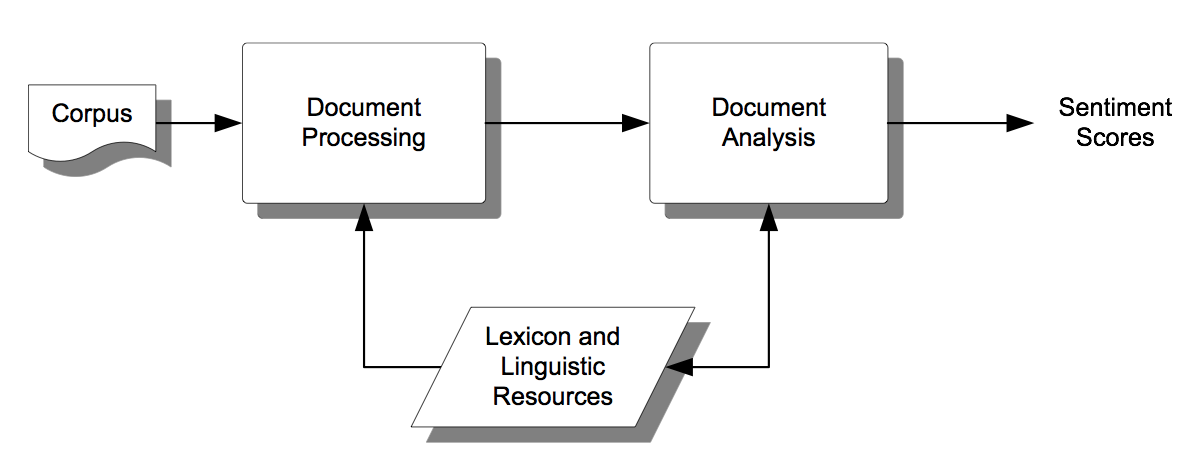
\includegraphics[scale=0.3]{Sentiment_001}
		\caption{The pipeline of modules in a generic sentiment analysis framework.}\label{fig:Sentiment_001}
	\end{figure}
	
	The input for a sentiment analysis framework is a corpus of documents, which may include a web page, news articles (which is particularly our case), a short post or a text document in any format. The corpus is pre-processed by document processing module, which converts corpus to texts by using linguistic resources for stemming, tokenization etc. Then pre-processed texts are sent to the document analysis module which annotates them using the linguistic resources and sometimes with a dictionary of words, called lexicon, which includes annotations of word's sentiment strength. The primary source of subjective content in a textual content can be adjectives (\cite{H1997}, \cite{H2004}), adverbs \cite{B2007}, adjectives and verbs \cite{K2004} or exclusive use of verbs \cite{S2008}. The output of the framework is the annotations which can be attached to whole document, to sentences, to entities as sentiment scores.
	
	The document analysis module, which is the main module of the framework, can apply two main lines of techniques for annotation: machine-learned and lexicon-based. In machine-learned sentiment analysis techniques \cite{P2002}, a model is built by a training dataset using common machine learning algorithms such as SVM, Naive Bayes, Logistics Regression, or KNN. Each document instance (e.g., a product review) in the dataset is associated with a value indicating the strength and polarity of the sentiments expressed in the text. In practice, obtaining large-scale labeled datasets is difficult, and the existing datasets are often domain-specific. As a remedy, the lexicon-based sentiment analysis techniques (\cite{B2010}, \cite{T2010}, \cite{TB2011}) aim to create a vocabulary and a set of rules to quantify the amount of sentiments in a given piece of text, eliminating the dependency to labeled training data. The vocabulary and rules are created manually, or by utilising resources like WordNet \cite{M1995}.
	
		
	\section{Structure of the work.}

	\begin{itemize}
		\item \textbf{Chapter \ref{introduction}} introduces the thesis, its goals and the current state of the art of \emph{Web Crawlers} and \emph{sentiment analysis}.
		\item \textbf{Chapter \ref{backgroundRelated}} presents the theoretical background needed in order to develop the technical and practical parts of the thesis. Besides in this chapter is presented the related work previously done in the field of news article analysis and its application to the stock markets.
		\item \textbf{Chapter \ref{analysisDesign}} introduces the analysis and design of the framework, this chapter is segmented in the design and analysis of the two main components: the \emph{news crawler} and the \emph{sentiment analysis}.
		\item \textbf{Chapter \ref{Realisation}} describe in detail how the framework was implemented, how to configure it, class diagram, data model and libraries used.
		\item \textbf{Chapter \ref{experimentalEvaluation}} shows experimentally how the multi-threading improved the performance of the framework, its thresholds with the available hardware. Besides we will make a simple analysis on the obtained data for \emph{the current most valuable company in history (so far)} \cite{BE2012}.
	\end{itemize}
	
	
.
	
	
	
	
	
	
	
		



